\section{Result}
\label{Result}
9 MCP PMTs were tested in testing system. The mean and standard deviation of parameters are calculated and shown in following sections.

\subsection{Gain, single PE resolution, P/V ratio, rise time, fall time and FWHM}
\begin{figure}[!htbp]
    \centering
    \begin{subfigure}[b]{0.49\textwidth}
        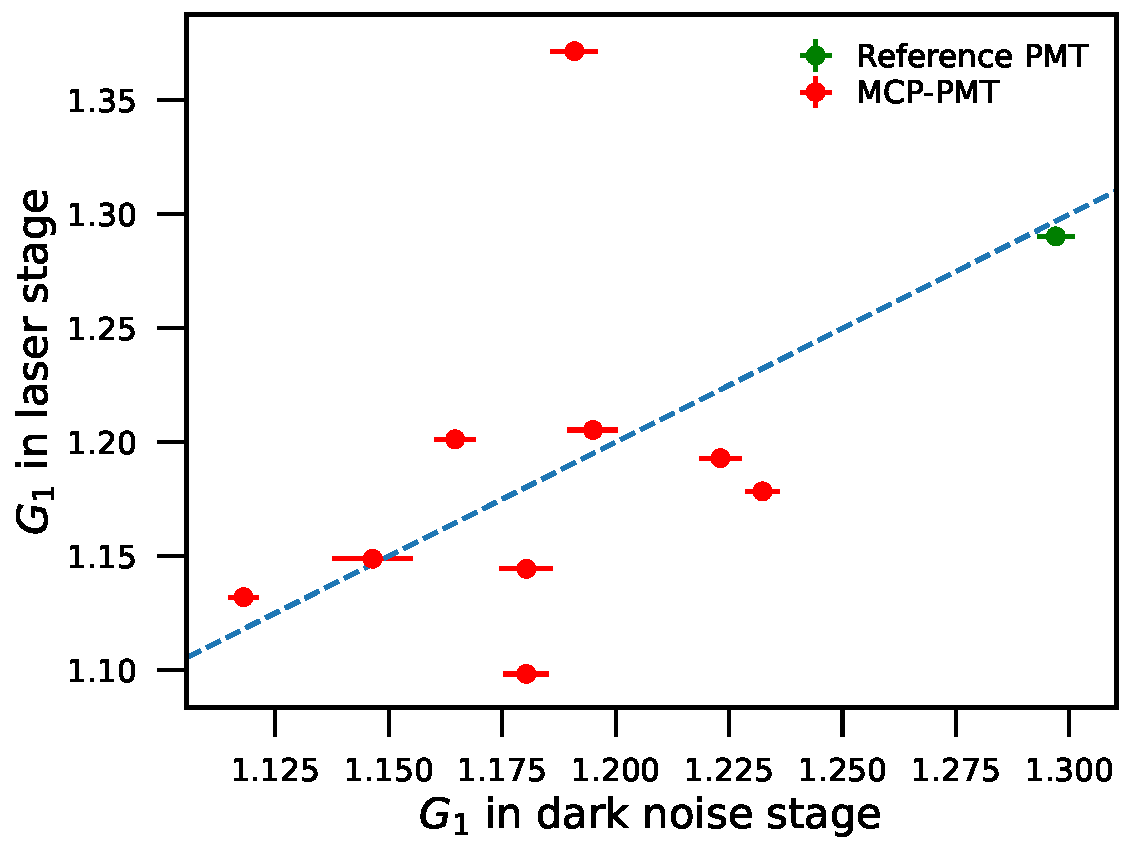
\includegraphics[width=\textwidth,page=1]{figures/result/compare.pdf}
        \caption{}
        \label{fig:gainCompare}
    \end{subfigure}
    \begin{subfigure}[b]{0.49\textwidth}
        \includegraphics[width=\textwidth,page=2]{figures/result/compare.pdf}
        \caption{}
        \label{fig:speresolutionCompare}
    \end{subfigure}
    \caption{(a) Gain of main peak of PMTs for noise and trigger stage. (b) Resolution of main peak for noise and trigger stage}
\end{figure}
Fig.~\ref{fig:gainCompare} and Fig.~\ref{fig:speresolutionCompare} indicates that the gain and single PE resolution of noise stage and trigger stage are consistent. Fig.~\ref{fig:totalchargeCompare} shows that mean of total charge $\mu_{C_t}$ is about 2 times of gain of main peak. The resolution of total charge in Fig.~\ref{fig:totalresolutionCompare} shows that the total charge resolution are close with reference PMT.

\begin{figure}
    \centering
    \begin{subfigure}[t]{0.49\textwidth}
        \includegraphics[width=\textwidth,page=3]{figures/result/compare.pdf}
        \caption{}
        \label{fig:totalchargeCompare}
    \end{subfigure}
    \begin{subfigure}[t]{0.49\textwidth}
        \includegraphics[width=\textwidth,page=4]{figures/result/compare.pdf}
        \caption{}
        \label{fig:totalresolutionCompare}
    \end{subfigure}
    \caption{(a) Gain of single PE $\mu_{C_t}$ for noise and trigger stage. (a) Resolution of single PE $\frac{\sigma_{C_t}}{\mu_{C_t}}$ for noise and trigger stage.}
\end{figure}

Due to the rate of trigger stage is larger than noise stage, the P/V ratio of trigger ratio is better than noise stage as shown in Fig.~\ref{fig:PVCompare}.
\begin{figure}[!htbp]
    \centering
    \begin{subfigure}[b]{0.49\textwidth}
        \includegraphics[width=\textwidth,page=5]{figures/result/compare.pdf}
        \caption{}
        \label{fig:PVCompare}
    \end{subfigure}
    \begin{subfigure}[b]{0.49\textwidth}
        \includegraphics[width=\textwidth,page=6]{figures/result/compare.pdf}
        \caption{}
        \label{fig:RiseCompare}
    \end{subfigure}
    \begin{subfigure}[b]{0.49\textwidth}
        \includegraphics[width=\textwidth,page=7]{figures/result/compare.pdf}
        \caption{}
        \label{fig:FallCompare}
    \end{subfigure}
    \begin{subfigure}[b]{0.49\textwidth}
        \includegraphics[width=\textwidth,page=8]{figures/result/compare.pdf}
        \caption{}
        \label{fig:FWHMCompare}
    \end{subfigure}
    \caption{(a) P/V ratio. (b) Rise time. (c) Fall time. (d) FWHM}
\end{figure}

As for time characteristics, the rise time, fall time, and FWHM are consistent between noise stage and trigger stage as shown in Fig.~\ref{fig:RiseCompare}, Fig.~\ref{fig:FallCompare}, and Fig.~\ref{fig:FWHMCompare}.

\subsection{DCR, relative PDE, and TTS}
The dark count rate and relative PDE of different MCP-PMTs are show in Fig.~\ref{fig:DCRCompare}. The mean DCR and mean PDE are \SI{}{kHz} and .
\begin{figure}[!htbp]
    \centering
    \begin{subfigure}[b]{0.49\textwidth}
        \includegraphics[width=\textwidth,page=9]{figures/result/compare.pdf}
        \caption{}
        \label{fig:DCRCompare}
    \end{subfigure}
    \begin{subfigure}[b]{0.49\textwidth}
        \includegraphics[width=\textwidth,page=10]{figures/result/compare.pdf}
        \caption{}
        \label{fig:TTSCompare}
    \end{subfigure}
    \caption{(a) DCR vs PDE (b) TTS results}
\end{figure}

The TTS of different MCP-PMTs are show in Fig.~\ref{fig:TTSCompare}. The mean TTS is \SI{}{ns}.


\subsection{Pre-pulse and after-pulse}
\begin{figure}[!htbp]
    \centering
    \begin{subfigure}[b]{0.49\textwidth}
        \includegraphics[width=\textwidth,page=11]{figures/result/compare.pdf}
        \caption{}
        \label{fig:prepulseCompare}
    \end{subfigure}
    \begin{subfigure}[b]{0.49\textwidth}
        \includegraphics[width=\textwidth,page=12]{figures/result/compare.pdf}
        \caption{}
        \label{fig:afterpulseCompare}
    \end{subfigure}
    \caption{(a) pre-pulse ratio. (b) after-pulse ratio.}
\end{figure}
Ratio of pre-pulse and after-pulse is .
\begin{figure}[!htbp]
    \centering
    \begin{subfigure}[b]{0.49\textwidth}
        \includegraphics[width=\textwidth,page=14]{figures/result/compare.pdf}
        \caption{}
        \label{fig:afterpulsePeak}
    \end{subfigure}
    \begin{subfigure}[b]{0.49\textwidth}
        \includegraphics[width=\textwidth,page=13]{figures/result/compare.pdf}
        \caption{$\sigma$}
        \label{fig:sigmaCompare}
    \end{subfigure}
    \caption{(a) Time and ratio of peaks of after pulse ratio. (b) $\tau$ and $\sigma$}
\end{figure}

\subsection{Paramerters of SER}
The mean $\tau$ and $\sigma$ of SER is \SI{}{ns} and \SI{}{ns}.
\subsection{Energy resolution boost}

Assume the number of expected photons $N$ on PMT is $\mu_N$ and obey poisson distribution $\pi~(\mu_N)$. Energy $E$ of Event proportional to $N=k\eta E$, in which $k$ is the factor which is relate to light yield and light transportation and $eta$ is the PDE of PMT. The phton detection efficiency of PMT is $\eta$ and the sigle PE charge distribution is Gaussian distribution $G(\mu_c,\sigma_c)$. The output charge distribution $C$ is hierachical model and the expectation and variance are
\begin{align}
    E[C]&=\mu_N\mu_c\\
    Var[C]&=\mu_c^2\mu_N+\mu_N\sigma_c^2
\end{align}
To be convenience, $N$ is estimated as $\hat{N}=\frac{C}{\mu_c}$ and $E$ is estimated as $\hat{E}=\frac{\hat{N}}{k}$. For event of energy $E$, the reconstructed energy resolution is 
\begin{equation}
    \frac{\sqrt{Var[\hat{E}]}}{E[\hat{E}]}=\frac{\sqrt{\mu_c^2\mu_N+\mu_N\sigma_c^2}}{\mu_N\mu_c}=\frac{\sqrt{1+(\frac{\sigma_c}{\mu_c})^2}}{\sqrt{\mu_N}}=\frac{\sqrt{1+(\frac{\sigma_c}{\mu_c})^2}}{\sqrt{k\eta E}}
\end{equation}

The energy resolution is dominated by sigle PE charge distribution, which is illustrated in the Fig.~\ref{fig:EnergyResolution}. Althogh there exist a long tail in charge distribution of MCP-PMT, $\frac{\sigma_c}{\mu_c}$ of MCP-PMT is better than reference PMT.
\begin{figure}[!htbp]
    \centering
    \includegraphics[width=0.7\textwidth,page=15]{figures/result/compare.pdf}
    \caption{Energy resolution}
    \label{fig:EnergyResolution}
\end{figure}